\chapter{Metodi e Modelli per lo sviluppo di applicazioni Mobile}
\lhead{\emph{Capitolo 2}}
Durante la mia esperienza presso la ditta BigThink SRL oltre ad una formazione pratica ho potuto, in alcuni momenti sotto la guida del capo azienda e del correlatore, studiare alcuni concetti teorici utili ad comprendere meglio le tecnologie utilizzate nel processo di sviluppo delle applicazioni in azienda. In questo capitolo si riportano dei concetti dell'informatica secondo me rilevanti(e alcune volte fondamentali) per lo sviluppo di applicazioni.

Una prima fase dello sviluppo è quella di strutturare l'architettura dell'applicazione e decidere come vengono assegnati i compiti. Una delle politiche che è stata intrapresa in azienda è stata quella della \emph{Separation of Concernes}(SoC), che in italiano si traduce in \emph{Separazione dei Compiti}. Si tratta di un principio di design per dividere un problema in sezioni distinte, e ad ogni sezione assegnare un particolare compito o risoluzione del problema. Questa scelta progettuale introduce il concetto di \emph{modulo} di una applicazione, atto a svolgere un certo compito dell'applicazione. I moduli ragionevolmente saranno indipendenti uno dall'altro in modo tale da garantirne l'integrità e il loro re-utilizzo.\cite{wiki:soc}\\

Il concetto appena visto astrae molto da una applicazione vera e propria, sta a chi la progetta decidere con che granularità  e se è veramente necessario applicarlo. Dato che parliamo di tecnologie web, un chiaro esempio si separazione dei compiti è quello della struttura di una pagina web, divisa in HTML per la struttura, CSS per lo stile, e Javascript per la logica e comportamento.\\

In questo capitolo andremo a vedere in che modo i compiti si possono separare all'interno di una applicazione, e quali strutture e/o design pattern possono risultare utili per lo sviluppo.
 
\section{Design Patterns}

Quando si progetta una applicazione risulta molto utile utilizzare schemi architetturali e metodologici che rendono da un lato l'applicazione efficiente dall'altro una scrittura del codice molto chiara e modulare, facile da correggere nel caso di eventuali errori. I design pattern vengono in aiuto a questa esigenza del programmatore.

\emph{In informatica, nell'ambito dell'ingegneria del software, un design pattern (traducibile in lingua italiana come schema progettuale, schema di progettazione, schema architetturale), è un concetto che può essere definito "una soluzione progettuale generale ad un problema ricorrente". Si tratta di una descrizione o modello logico da applicare per la risoluzione di un problema che può presentarsi in diverse situazioni durante le fasi di progettazione e sviluppo del software, ancor prima della definizione dell'algoritmo risolutivo della parte computazionale.}
\hspace*{\fill}\cite{wiki:design_pattern} 

Il problema ricorrente che si ha nello sviluppo di applicazioni e quello della decisione di dove debbano stare determinati compiti / operazioni / sezioni all'interno dell'applicazione. Ad esempio la separazione della parte dell'interfaccia da quella dedicata alla manipolazione dei dati da quella dedicata alla memorizzazione. Dividere i vari compiti di una applicazione può risultare molto produttivo, in quanto si possono sviluppare in parallelo diverse parti dell'applicazione senza influire sulle altre e volendo con la possibilità di utilizzare tecnologie differenti.

Durante il periodo di tirocinio presso l'azienda \emph{BigThink SRL} per la creazione di Web Applications sono stati utilizzati pattern come : Client-Server, SoC, Frontend e Backend, MVC; gli altri design pattern che verranno introdotti sono necessari per comprendere meglio alcune tecnologie che verranno utilizzate.
 
\subsection{Frontend e Backend}
Queste due parole sono spesso usate in informatica in molti ambiti, nel contesto specifico dell'applicazione \texttt{frontend}(in italiano parte davanti) denota quella parte dell'applicazione responsabile di gestire l'interfaccia utente e i dati provenienti da essa, mentre \texttt{backend}(in italiano parte dietro) indica la sezione dell'applicazione dedita alla gestione dei dati dell'applicazione. L'interazione che hanno le due parti è un chiaro esempio di interfaccia.\\

\textbf{Frontend:} questa è la parte caratteristica dell'applicazione, in quanto ne definisce il comportamento e l'aspetto, determinando la logica con cui si evolverà al rapporto con l'utente. A differenza della parte \emph{backend} questa non definisce ne manipolazione, ne la rappresentazione dei dati ma la vista che ha l'utente su di essi. Nella parte \emph{frontend} è inclusa anche la fase di definizione estetica dell'interfaccia, ma spesso questa spetta a una figura professionale distinta atta "vestire" l'applicazione.\\

\textbf{Backend:} questa parte è completamente diversa dalla prima, in quanto definisce la manipolazione dei dati all'interno dell'applicazione. In particolare fornisce dei servizi / risorse ai quali la parte \emph{frontend} può accedere e effettuare delle operazioni, come ad esempio l'autenticazione di un utente a un servizio. Tutta la gestione dei dati che viene fatta da questa parte, viene oscurata alla parte \emph{frontend} per garantire un servizio di sicurezza molto elementare, in modo tale che se l'utente inserisce dei dati errati che vengono passati dalla parte \emph{frontend} a quella \emph{backend}, nessuna operazione verrà eseguita e l'integrità dei dati verrà preservata.\\

Si tratta di una separazione concettuale e non fisica delle parti, accade spesso che si facciano analogie con il pattern client-server(spiegato successivamente); le due parti possono anche risiedere sullo stesso dispositivo / calcolatore.

A livello professionale molti sviluppatori si identificano appunto come \emph{frontend} e/o \emph{backend} developer ovvero specializzati nello sviluppo di una parte specifica dell'applicazione. Se la parte \emph{backend} viene progettata secondo dei corretti schemi, e possibile riutilizzare le risorse anche in futuro, purché si rispetti l'interfaccia. Inoltre a livello professionale si può procedere parallelamente nello sviluppo delle parti in modo tale da ottimizzare i tempi, pur seguendo uno schema stabilito a priori.\\

\subsection{Pattern Client-Server}
\label{subsec:Client-Server}

In uno schema di applicazione su larga scala può risultare utile separare le parti logiche dell'applicazione su entità diverse che poi saranno messe in comunicazione. Ad esempio la computazione di un certo processo di calcolo potrebbe risultare molto onerosa a livello di prestazioni e che un dispositivo mobile possa non essere in grado supportarla. A questo punto risulta conveniente adottare una architettura client-server dove è il server che si occupa di eseguire le operazioni di calcolo mentre il client di rappresentare l'output. 

\textbf{Definizione:} Il modello client-server è un modo per strutturare applicazioni distribuite che distingue due parti di un processo di comunicazione, la prima che fornisce una risorsa e/o un servizio chiamata server, la seconda che analogamente li può richiedere, chiamata client. La comunicazione in generale avviene attraverso la rete, ed è il client a iniziarla. Il compito del server è quello di predisporre le risorse che ha ai vari client che li chiedono, rimanendo appunto "in ascolto", il client invece non condivide le risorse con altri, può solo interagire con il server\cite{wiki:cliserv}.\\

La divisione client e server associata con le parti frontend e backend di una applicazione viene spesso utilizzata nello sviluppo di applicazioni mobile distribuite, ad esempio in servizi georeferenziati. Ma non e detto che in generale sia sempre la soluzione ottima da adottare. 

\subsection{MVC Pattern}
\label{sec:MVC}

L'evoluzione della complessità del codice delle applicazioni, ha fatto si che i programmatori adottassero strategie di scrittura del codice in modo che rimanesse mantenibile e riusabile. L'uso del pattern MVC ha trovato largo uso in molti framework Javascript in modo tale che il codice scritto dal programmatore ereditasse i suoi benefici. Questa logica inoltre nello sviluppo complessivo dell'applicazione ha fatto si che il programmatore potesse disporre di uno scheletro dell'applicazione generico, in modo tale da accelerare il processo di sviluppo e di disporre di eventuali parti già sviluppate.

\emph{Il Model-View-Controller pattern (MVC) in informatica, è un pattern architetturale molto diffuso nello sviluppo di sistemi software, in particolare nell'ambito della programmazione orientata agli oggetti, in grado di separare la logica di presentazione dei dati dalla logica di business.}

\begin{figure}[htbp]
  \centering
    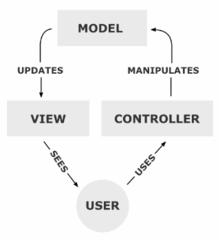
\includegraphics[scale=0.75]{Figures/mvc.png}  
    \rule{35em}{0.5pt}
  \caption[MVC Pattern]{Schema del pattern MVC}
  \label{fig:MVC Schema}
\end{figure}

Il pattern è basato sulla separazione dei compiti fra i componenti software che interpretano tre ruoli principali:
\begin{description}
\item[model] fornisce i metodi per accedere ai dati utili all'applicazione;
\item[view] visualizza i dati contenuti nel model e si occupa dell'interazione con utenti e agenti;
\item[controller] riceve i comandi dell'utente (in genere attraverso il view) e li attua modificando lo stato degli altri due componenti.
\end{description}
Questo schema, fra l'altro, implica anche la tradizionale separazione fra la logica applicativa (in questo contesto spesso chiamata "logica di business"), a carico del controller e del model, e l'interfaccia utente a carico del view.
\hspace*{\fill}\cite{wiki:mvc}

Il framework AngularJS spiegato nella sezione \ref{sec:AngularJS} è sviluppato secondo questo pattern. Il concetto verrà inoltre richiamato nella spiegazione di altri processi di sviluppo. 

\subsection{MVVM Pattern}

Nello sviluppo di applicazioni mobile si avrà a che fare con il concetto di vista e di modello che rispettivamente denotano l'interfaccia utente e i dati che vengono mostrati sulla vista(si vedrà perché intesi come modelli). Nell'ottica di tenere la logica dell'applicazione separata dalla rappresentazione dei dati il pattern MVVM detta le linee guida per poter scrivere codice che tenga conto di questi aspetti.

\emph{Il Model-View-ViewModel è un pattern architetturale basato sul pattern MVC e MVP che tenta di separare più chiaramente lo sviluppo di interfacce utente (UI) da quello della logica di business e il comportamento in un'applicazione . A tal fine, molte implementazioni di questo modello fanno uso di associazioni dati dichiarativa(data bindings) per consentire una separazione di lavoro su Vista da altri livelli.}
\hspace*{\fill}\cite{book:mvvm}

\begin{figure}[htbp]
  \centering
    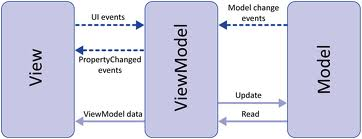
\includegraphics[scale=0.75]{Figures/mvvm-1.jpeg}  
    \rule{35em}{0.5pt}
  \caption[MVVM Pattern]{Schema del pattern MVVM}
  \label{fig:MVVM Schema}
\end{figure}

Il fulcro del funzionamento di questo pattern è la creazione di un componente, il ViewModel appunto, che rappresenta tutte le informazioni e i comportamenti della vista corrispondente. La vista si limita infatti, a visualizzare graficamente quanto esposto dal ViewModel, a riflettere in esso i suoi cambi di stato oppure ad attivarne dei comportamenti.

Questo facilita l'interfaccia utente e lo sviluppo che si verificano quasi contemporaneamente all'interno dello stesso codice. Gli sviluppatori dell'interfaccia utente scrivono associazioni verso il ViewModel nel documento di markup (HTML) mentre il Model e il ViewModel sono mantenuti da altri sviluppatori che lavorano sulla logica dell'applicazione(business logic).

\section{API}

\emph{In informatica le API(Application Programming Interface) sono un insieme di operazioni, protocolli, strumenti per lo sviluppo del software. Una API rappresenta una specifica componente del software in termini di operazione, input, output e tipi soggiacenti. Una API definisce funzionalità totalmente indipendenti dalla loro rispettiva implementazione, il che consente di poter variare rispettivamente l'implementazione e la definizione senza che una influisca sull'altra. Una buona API rende più facile lo sviluppo del software fornendo vari "mattoni" con cui poter sviluppare il software, il ruolo del programmatore è quello di unire i vari blocchi richiesti.}
\hspace*{\fill}\cite{wiki:api}

Un primo esempio di API è già stato menzionato quando si è parlato dei framework per lo sviluppo ibrido. In quel caso le API erano fornite tramite Javascript in modo tale che potessero essere interpretate all'interno di un contenitore nativo che potesse interpretare linguaggi web(come un browser). In questo caso i blocchi di cui si parla sono le rispettive API che consentono di comunicare con le funzionalità del dispositivo come ad esempio la fotocamera, il gps, la vibrazione, l'accelerometro ecc\ldots.

L'utilizzo di API è stato fatto durante il mio tirocinio aziendale per lo scambio di dati tra la parte Frontend e Backend di Web Application, in particolare sono state utilizzate delle API REST.

\subsection{API Rest}

REST(\textbf{R}epresentational \textbf{S}tate \textbf{T}ransfer) è un termine coniato da Roy Fieldin(co-autore del protocollo HTTP 1.1) nella sua tesi di dottorato per descrivere lo stile dell'architettura dei sistemi di rete. REST non è un protocollo e nemmeno uno standard, ma uno \emph{stile} architetturale per applicazioni / servizi web; quando uno di essi rispetta i criteri di REST gli si da l'attributo \emph{RESTful}.

REST impone determinati vincoli alla sua architettura, pur lasciando libera la loro implementazione:

\begin{description}

\item[Uniform Interface] 

REST impone una interfaccia uniforme tra client e server. Questo semplifica e decompone l'architettura, il che fa si che ogni parte possa evolvere indipendentemente. Per creare una interfaccia uniforme si sono 4 principi da seguire:

\item[- Resource Based] 

ogni risorsa deve essere identificata univocamente all'interno del server. La sua identificazione deve essere concettualmente separata dalla rappresentazione che viene ritornata al client, la quale può dipendere dalla richiesta fatta.

\item[- Manipolazione delle Risorse] 

il client tramite il riferimento della risorsa può effettuare 4 operazioni base creazione, lettura, aggiornamento, cancellazione (\emph{CRUD}: \textbf{C}reate \textbf{R}ead \textbf{U}pdate \textbf{D}elete)

\item[- Self-descriptive Messages] 

Ogni messaggio tra client e server contiene tutte le informazioni sufficienti per la sua codifica e interpretazione. Le risposte dal server devono indicare anche i parametri di caching.

\item[- Hypermedia as the Engine of Application State (HATEOAS)] 
\label{itm:hateoas}
Uno dei principi REST suggerisce l'uso di collegamenti tra risorse come modalità di transizione da uno stato all'altro. Questo principio è noto anche con l'acronimo HATEOAS, Hypermedia As The Engine Of Application State, e focalizza l'attenzione sull'utilizzo dei collegamenti ipertestuali, anzi ipermediali, come meccanismo di base per far passare un'applicazione da uno stato ad un altro.
Se il risultato di una interazione con il server è un contenitore di risorse, allora all’interno della risorsa abbiamo gli URI delle risorse contenute, altrimenti nella maggior parte dei casi non si hanno altri collegamenti. Non possiamo dire che un Web Service di questo tipo non sia RESTful, ma nella maggior parte dei casi non sfrutta a pieno le potenzialità dei principi REST.
Il principio HATEOAS, infatti, intende incoraggiare non solo l’uso di collegamenti per rappresentare risorse composte, ma anche per definire qualsiasi altra relazione tra le risorse e per controllare le transizioni ammissibili tra uno stato e l’altro dell’applicazione.
Sfruttando pienamente il principio HATEOAS è possibile creare servizi Web con scarso accoppiamento tra client e server. Infatti, se il server riorganizza le relazioni tra le risorse, il client è in grado di trovare tutto ciò che serve nelle rappresentazioni ricevute. Potenzialmente tutto quello che servirebbe ad un client è solo l’URI della risorsa iniziale. Come avanzare tra uno stato e l’altro dell’applicazione verrà indicato man mano che si seguono i collegamenti incorporati nelle successive rappresentazioni di risorse.
\hspace*{\fill}\cite{web:hateoas}

\item[Stateless]

La parte \emph{State} dell'acronimo di REST, sta a indicare un architettura di rete che non mantiene lo stato della risorsa. Ovvero lo stato della risorsa viene passato tramite il corpo del messaggio che viene scambiato tra client e server. Essendo ogni risorsa identificata con un URI(\textbf{U}niversal \textbf{R}esource \textbf{I}dentificator), quando viene fatta una richiesta alla risorsa può avvenire un cambiamento di stato di quest'ultima. In qualunque caso lo stato finale della risorsa viene comunicato al client nel corpo del messaggio di risposta.

Nell'industria delle reti si può ricordare il concetto di \emph{sessione} HTTP, ovvero dove lo stato di una risorsa viene mantenuto attraverso richieste HTTP multiple. Nel caso di REST, il client si deve preoccupare di includere tutte le informazioni necessarie nella richiesta al server, e nel caso di richieste multiple è obbligato a inviare in tutte le richieste lo stato aggiornato della risorsa. Questo permette di far si che i server non debbano preoccupare di mantenere lo stato delle loro risorse, in modo tale da garantire una maggiore scalabilità del sistema.

Quindi la differenza tra stato e risorsa è che: lo stato o lo stato di una applicazione, e ciò a cui importa al server per soddisfare la richiesta corrente. Una risorsa o lo stato di una risorsa sono i dati che definiscono la rappresentazione della risorsa.
Per essere più chiari si consideri lo stato dell'applicazione come i dati nella richiesta che possono variare da client a client. Mentre lo stato della risorsa rimane costante dipendentemente da ogni client che la richiede.

\item[Cacheadable]

Nel World Wide Web i client possono mantenere una cache delle richieste fatte ai server. In una architettura REST le richieste devono specificare, esplicitamente o implicitamente, la possibilità di essere mantenute in cache oppure no, per prevenire ai client di ri-usare stati o dati inappropiati per richieste future. Una buona gestione della cache può parzialmente o completamente eliminare alcune interazioni tra client e server, così da migliorare prestazioni e scalabilità.

\item[Client-Server]  

La struttura dell'applicazione deve essere di tipo client-server, mostrata nella sezione \ref{subsec:Client-Server}. Avendo una interfaccia uniforme, in una architettura REST i client sono separati dai server. Questo fa si che ci sia una separazione dei compiti tra i due, ad esempio: i client non hanno la visione su come i dati vengono memorizzati, il quale compito spetta al server.In questo modo migliora la portabilità del codice del client, mentre i server non sono a conoscenza di come sia fatta l'interfaccia utente del client. Questo fa si che i la logica del server sia più semplice e scalabile. Se l'interfaccia tra client e server non viene alterata, le due entità possono venire sviluppate o sostituite in modo del tutto indipendente.  

\item[Layered system]

Avere un sistema a livelli può migliorare la scalabilità, la distribuzione del carico di lavoro e cache condivise, in quanto un client non potrà mai sapere se e connesso a un intermediario o direttamente al server. I server intermediari possono garantire tutti i miglioramenti prima nominati con la possibilità di adottare anche una politica di sicurezza.

\item[Code on demand(OPTIONAL)]

Un parametro opzionale di una architettura REST è la possibilità dei server di estendere le capacità dei client trasferendo una determinata logica che può essere eseguita a destinazione.

\end{description}

\subsubsection{Implementazioni Esistenti}

Un protocollo di comunicazione utilizzato nelle reti che si presta ad essere molto compatibile con una architettura di tipo REST e sicuramente HTTP. Spesso il protocollo e l'architettura vengono mischiati all'interno della spiegazione di che cosa è REST, si tiene a precisare che l'architettura REST può essere applicata anche in un sistema che non fa uso di HTTP in quanto si tratta di una architettura che specifica il modo in cui client e server devono comunicare ma lascia libera l'implementazione del sistema.

Il 99\% delle applicazioni RESTful viene usato il protocollo HTTP in quanto è già possibile associare i verbi dell'architettura REST con le richieste del protocollo: 
\begin{itemize}
\item CREATE $\Rightarrow$ POST, crea una nuova risorsa

\item READ   $\Rightarrow$ GET, ottiene una risorsa specifica

\item UPDATE $\Rightarrow$ PUT, modifica una risorsa specifica

\item DELETE $\Rightarrow$ DELETE, elimina una risorsa specifica

\end{itemize}
Inoltre tramite il \emph{payload} di HTTP è possibile scambiare tra client e server lo stato delle risorse e la relativa rappresentazione dati.

Il protocollo HTTP identifica le risorse tramite un \textbf{URL}(\textbf{U}niversal \textbf{R}esource \textbf{L}ocator) e garantisce all'architettura REST un modo per accedere univocamente alle risorse.
Prima che le applicazioni cominciassero ad essere sviluppate secondo una architettura REST, non c'erano vincoli su come una richiesta a una determinata risorsa doveva essere effettuata il che rendeva l'identificazione delle risorse poco chiara.
\begin{lstlisting}[caption={Esempio di URL che non rispetta il vincolo di REST}, label={lst:wrongRESTURL}]
	GET index.php?service=getUser&id=55
\end{lstlisting}
Nell'esempio \ref{lst:wrongRESTURL} notiamo che l'URL non denota una specifica risorsa nel sever ma il metodo e i parametri che il server dovrà utilizzare per comporre il risultato e rispondere alla richiesta. Questo metodo non è errato ma non va bene per identificare delle risorse.
In una architettura REST le risorse vengono identificate secondo precisi URL univoci all'interno dell'applicazione, come nell'esempio \ref{lst:correctRESTURL}.
Inoltre è buona pratica creare identificatori di risorse gerarchici, in modo da rendere l'URL della risorsa chiaro e semplice da comprendere.

\begin{lstlisting}[caption={Identificazione di una risorsa all'interno di una architettura REST}, label={lst:correctRESTURL}]
	GET /api/user/55
\end{lstlisting}

Per quanto riguarda la rappresentazione dei dati nello scambio di risorse, i formati più utilizzati sono JSON(\textbf{J}ava\textbf{S}cript \textbf{O}bject \textbf{N}otation) e XML(e\textbf{X}tensible \textbf{M}arkup \textbf{L}anguage) i quali permettono una struttura dettagliata e gerarchica dei dati. Nelle applicazioni web viene utilizzato maggiormente JSON in quanto la sua manipolazione risulta più diretta nel linguaggio Javascript.

La domanda che ora sorge spontanea è: come si creano delle \textbf{buone} API REST? Roy Fielding in suo articolo condanna l'uso dell'attributo RESTful su applicazioni che in realtà lo sono solo in parte, in quanto per far si che lo siano \textbf{tutti} i vincoli dell'architettura REST devono essere rispettati.
Uno di questi che viene spesso trascurato e HATEOAS(\ref{itm:hateoas}) e l'inventore di REST reclama i principi di come dovrebbero essere sviluppate correttamente delle API REST in questo articolo \citep{web:restapi}

%\begin{itemize}
%
%\item Una API REST non deve dipendere dal protocollo di comunicazione. E in generale ogni protocollo che utilizza degli URI deve permettere di usare un qualsiasi schema di quest'ultimo per l'identificazione dellea risorsa. Se questo punto viene meno l'identificazione delle risorse non è separata  dalla loro interazione.
%
%\item Una API REST non deve contenere cambiamenti inerenti al protocollo, è consentito soltanto modificare i bit che il quest'ultimo mette a disposizione. Se non si rispetta questo vincolo l'interfaccia alla risora diventa specifica e non generica.
%
%\item Una API REST dovrebbe descrivere accuratamente i tipi ipermediali utilizzati per rappresentare la risorsa(HATEOAS) e lo stato dell'applicazione.
%
%\item Una API REST non deve fissare il nome di una risorsa e la sua gerarchia. I server devono avere la libertà di poter cambiare la loro namespace. Avere dei nomi fissi rende l'architettura equivalente ad una applicazione RPC.
%
%\item Una API REST non deve avere risorse di un tipo significativo per il client. Gli unici tipi significativi per il client sono la rappresentazione corrente dei tipi multimediali e in nomi delle relazioni standardizzati.
%
%\item Una API REST 
%\end{itemize}

\subsubsection{CORS}

Si è parlato precedentemente della comunicazione tra client e server risiedenti su macchine differenti. Accade spesso che queste due entità siano situate su domini internet diversi e che la richiesta debba transitare da uno all'altro. CORS(\textbf{C}ross \textbf{O}rigin \textbf{R}esource \textbf{S}haring) è uno standard W3C che regolamenta le richieste di risorse tra domini differenti. È stato adottato per garantire un livello di sicurezza per l'accesso alle risorse. Per poterlo utilizzare bisogna agire sulla configurazione del server e sugli header dei messaggi HTTP.
Ad esempio il dominio \emph{www.marcopredari.it} vuole richiedere una risorsa presso \emph{www.google.it}. Innanzitutto il dominio chiamante deve aggiungere all'header il campo \textbf{Origin} indicando il prorpio dominio. Come risposta riceverà un messaggio il cui header avrà all'interno il campo \textit{Allow-Control-Allow-Origin} contenete i domini abilitati a richiedere quella risorsa; nel caso del simbolo * significa che accetta qualsiasi dominio la richieda. Se il dominio che fatto la richiesta non fosse autorizzato riceverà un messaggio di errore. \cite{web:cors}

\begin{lstlisting}[caption={esempio di richiesta HTTP utilizzando CORS}, label={lst:CORSrequest}]
	Accept:application/json, text/plain, */*
	Accept-Encoding:gzip, deflate, sdch
	Accept-Language:it-IT,it;q=0.8,en-US;q=0.6,en;q=0.4
	Cache-Control:no-cache
	Connection:keep-alive
	Host:predoweb-cms.herokuapp.com
	Origin:http://127.0.0.1
	Pragma:no-cache
	Referer:http://127.0.0.1/webcv/blog.marcopredari.it/
	User-Agent: Mozilla/5.0 (X11; Linux x86_64) 
			    AppleWebKit/537.36 (KHTML, like Gecko) 
			    Chrome/39.0.2171.99 Safari/537.36
\end{lstlisting}
\begin{lstlisting}[caption={esempio di risposta dal server che utilizza CORS}, label={lst:CORSanswer}]
	Access-Control-Allow-Origin:http://127.0.0.1
	Cache-Control:no-cache
	Connection:keep-alive
	Content-Type:application/json
	Date:Tue, 20 Jan 2015 16:52:13 GMT
	Server:Apache/2.4.10 (Unix)
	Set-Cookie:laravel_session= .....
			   expires=Tue, 20-Jan-2015 18:52:13 GMT; 
			   Max-Age=7200; 
			   path=/; 
			   httponly
	Transfer-Encoding:chunked
	Vary:Origin
	Via:1.1 vegur
	X-Frame-Options:SAMEORIGIN
	X-Powered-By:PHP/5.6.4
\end{lstlisting}

CORS possiede inoltre altre configurazioni riguardo alla sicurezza delle richieste, nei web server come Apache è possibile configurare un file in cui si possono aggiungere tutte le restrizioni o concessioni del caso.

%Scaletta REST
%
%- origini / storia: Com'è nato REST?
%- cosa cerca di risolvere REST
%- Come lo risolve: parte teorica
%	- Le risorse
%	- Operazioni sulle risorse: I verbi
%	- Concetto di applicazione RESTFul
%    - HTTP e REST
%- Implementazioni esistenti
%	- Differenza con il passato
%    GET api/users/10
%    POST pippo/pluto/10/topolino
%    			= 
%    POST index.php?route=pippo/pluto/10/topolino
%    
%    GET index.php?service=get_user&id=10
%	- Servizi Backend (più o meno tutti i linguaggi esistenti)
%    	- gateway: Single entry point -> pagina che fa da gateway alle richieste e fa una sorta di traduzione
%    	- URL Rewriting  : mettere a disposizione delle risorse o dei servizi tramite URL
%    - Frontend 
%    	- Chiamate HTTP XHR (GET/POST/PUT/DELETE)
%        - JSON parsing / XML Parsing / other
% - CORS
%  	- Definizione -> a cosa serve ?
%    - Esempi di implementazioni (Aggiunta dell'header)

